\section{Seq2Seq Architecture}
\begin{frame}{}
  \LARGE \textbf{Seq2Seq Architecture}
\end{frame}

\begin{frame}{Seq2Seq Architecture}
  \textbf{Key Idea:} Map input sequence $\rightarrow$ intermediate vector $\rightarrow$ output sequence.
  \vspace{1em}
  \begin{itemize}
    \item[\textcolor{red}{$\blacktriangleright$}] \textbf{Encoder RNN:} Processes input sequence and compresses it into a \textbf{fixed-length vector} (context).
    \item[\textcolor{red}{$\blacktriangleright$}] \textbf{Decoder RNN:} Generates output sequence from the context vector.
  \end{itemize}
  \vspace{1em}
  \textbf{Applications:}
  \begin{itemize}
    \item[\textcolor{red}{$\blacktriangleright$}] Machine translation
    \item[\textcolor{red}{$\blacktriangleright$}] Summarization
    \item[\textcolor{red}{$\blacktriangleright$}] Dialogue systems
    \item[\textcolor{red}{$\blacktriangleright$}] Speech recognition
  \end{itemize}
\end{frame}

\begin{frame}{Seq2Seq Architecture}
  \centering
  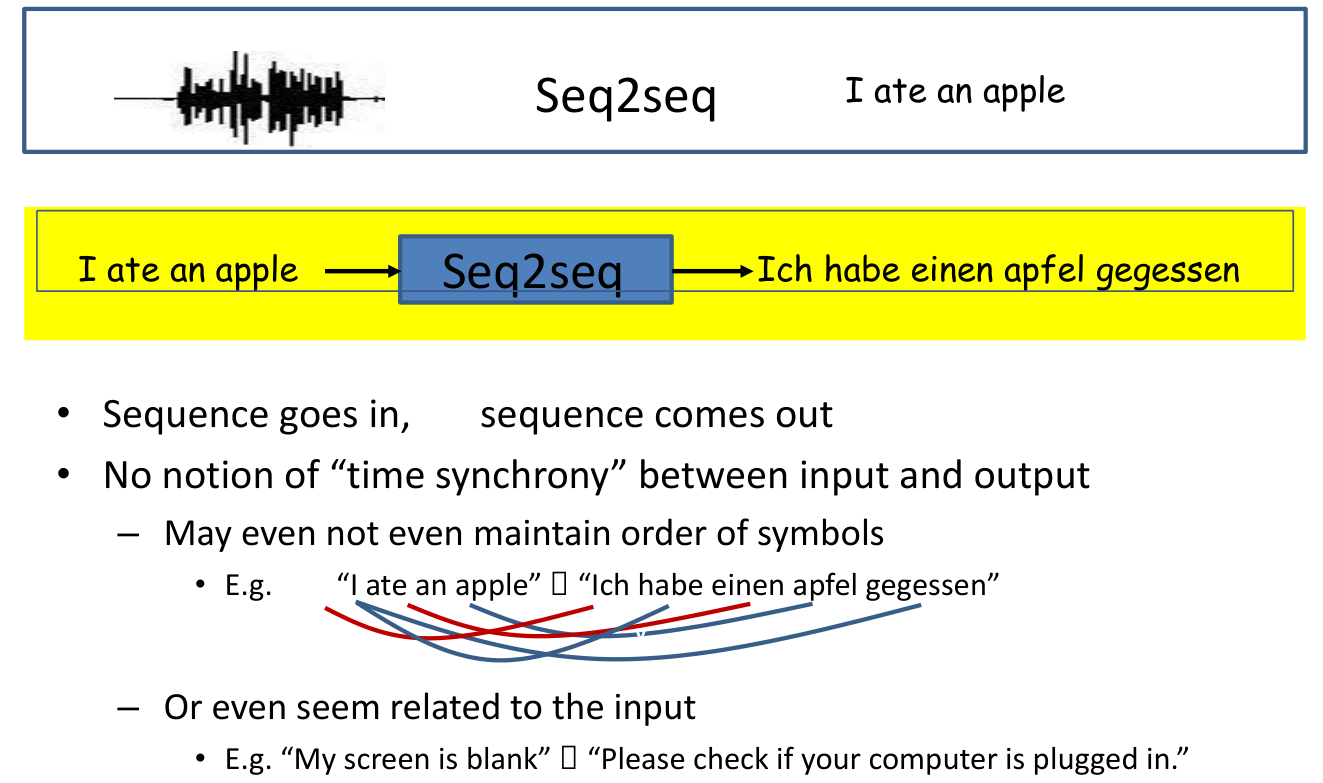
\includegraphics[width=0.35\paperwidth,height=0.35\paperheight,keepaspectratio]{images/seq2seq+attention/seq2seq_overview_speech_translation.png}

  {\scriptsize Source: after CMU 11-785 (Spring 2024), Lecture 18: Sequence to Sequence Models \& Attention, slide~2.}
\end{frame}

\begin{frame}{Modeling the problem}
  \centering
  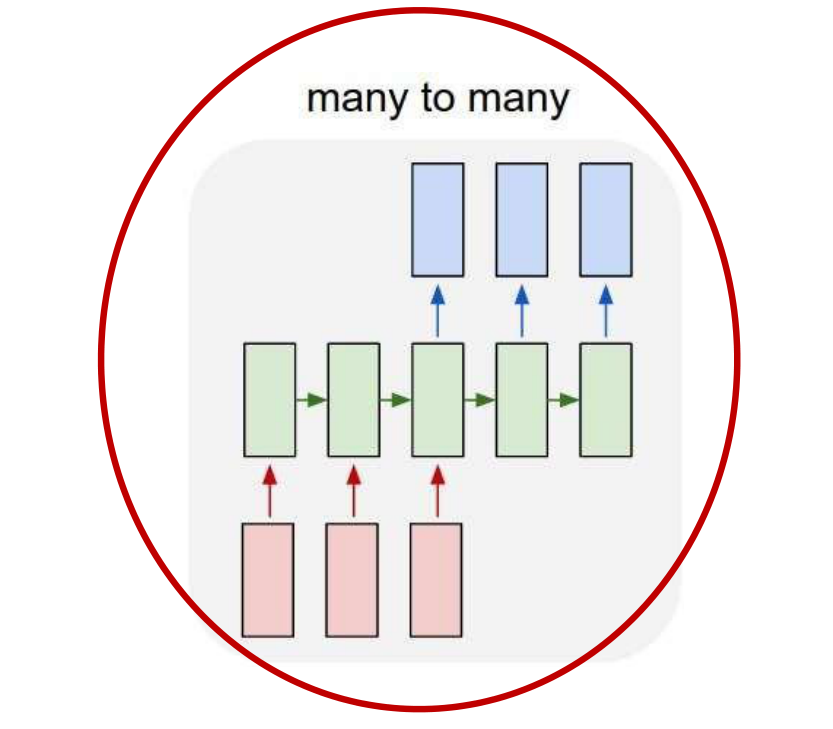
\includegraphics[width=0.35\paperwidth,height=0.35\paperheight,keepaspectratio]{images/seq2seq+attention/seq2seq_many_to_many_rnn.png}

  {\scriptsize Source: after CMU 11-785 (Spring 2024), Lecture 18: Sequence to Sequence Models \& Attention, slide~3 (RNN-taxonomy panel after A. Karpathy, 2015).}

  \centering
  \textit{Delayed} sequence to sequence
\end{frame}

\begin{frame}{Modeling the problem}
  \centering
  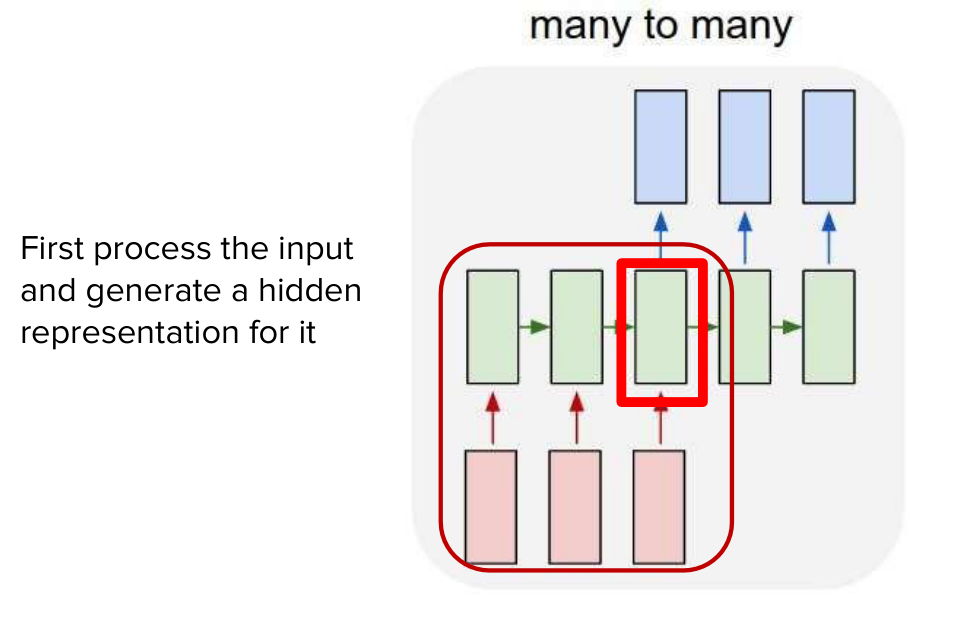
\includegraphics[width=0.35\paperwidth,height=0.35\paperheight,keepaspectratio]{images/seq2seq+attention/seq2seq_encoder_process_input.png}

  {\scriptsize Source: after CMU 11-785 (Spring 2024), Lecture 18: Sequence to Sequence Models \& Attention, slide~4 (RNN-taxonomy panel after A. Karpathy, 2015).}

  \centering
  \LARGE \textit{Delayed} sequence to sequence
\end{frame}

\begin{frame}{Modeling the problem}
  \centering
  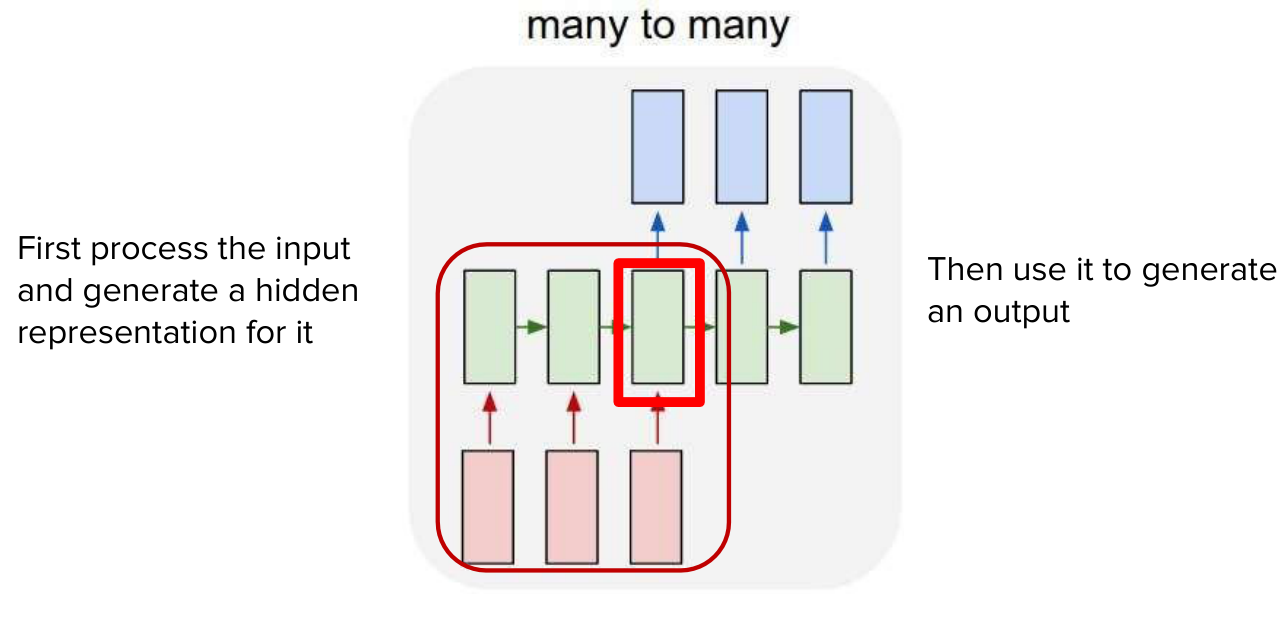
\includegraphics[width=0.35\paperwidth,height=0.35\paperheight,keepaspectratio]{images/seq2seq+attention/seq2seq_encoder_then_decoder.png}

  {\scriptsize Source: after CMU 11-785 (Spring 2024), Lecture 18: Sequence to Sequence Models \& Attention, slide~5 (RNN-taxonomy panel after A. Karpathy, 2015).}

  \LARGE \textit{Delayed} sequence to sequence
\end{frame}

\begin{frame}{Modeling the problem}
  \centering
  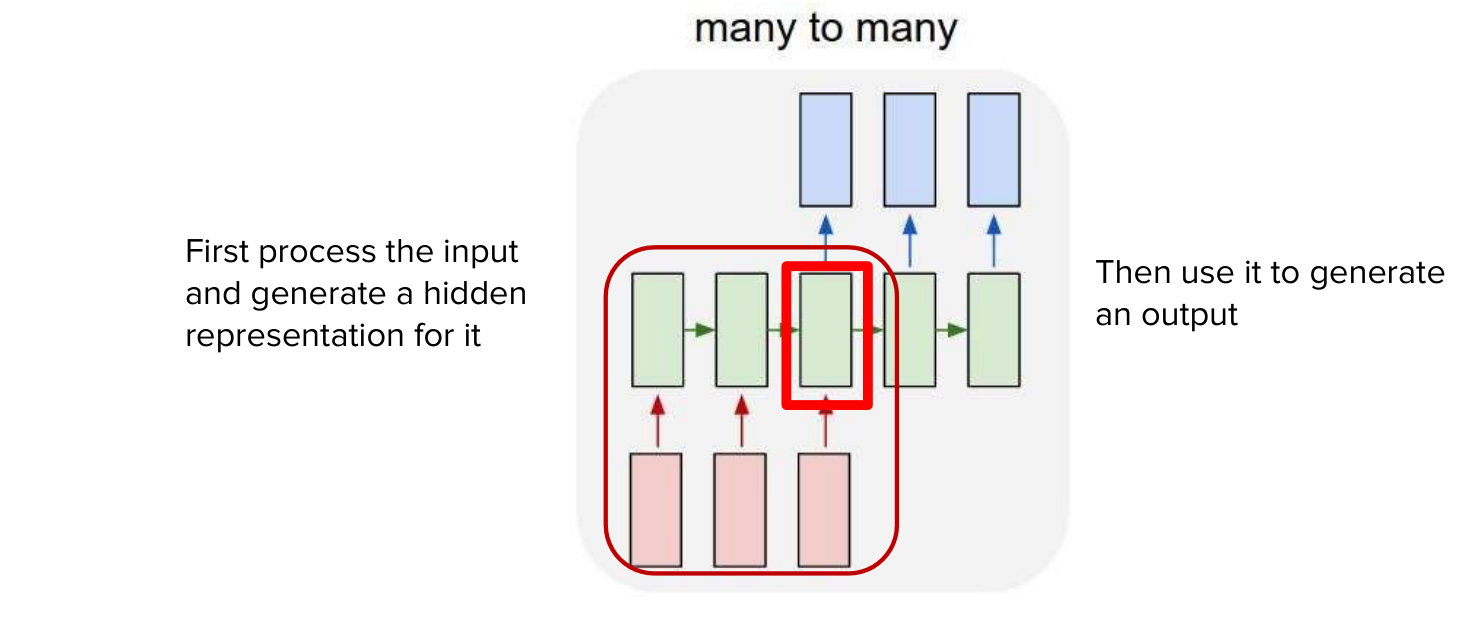
\includegraphics[width=0.35\paperwidth,height=0.35\paperheight,keepaspectratio]{images/seq2seq+attention/seq2seq_encoder_decoder_split.png}

  {\scriptsize Source: after CMU 11-785 (Spring 2024), Lecture 18: Sequence to Sequence Models \& Attention, slide~6 (RNN-taxonomy panel after A. Karpathy, 2015).}

  \textit{Problem:} Each word that is output depends only on  current hidden state, and not on previous outputs
\end{frame}

\begin{frame}{Modeling the problem}
  \centering
  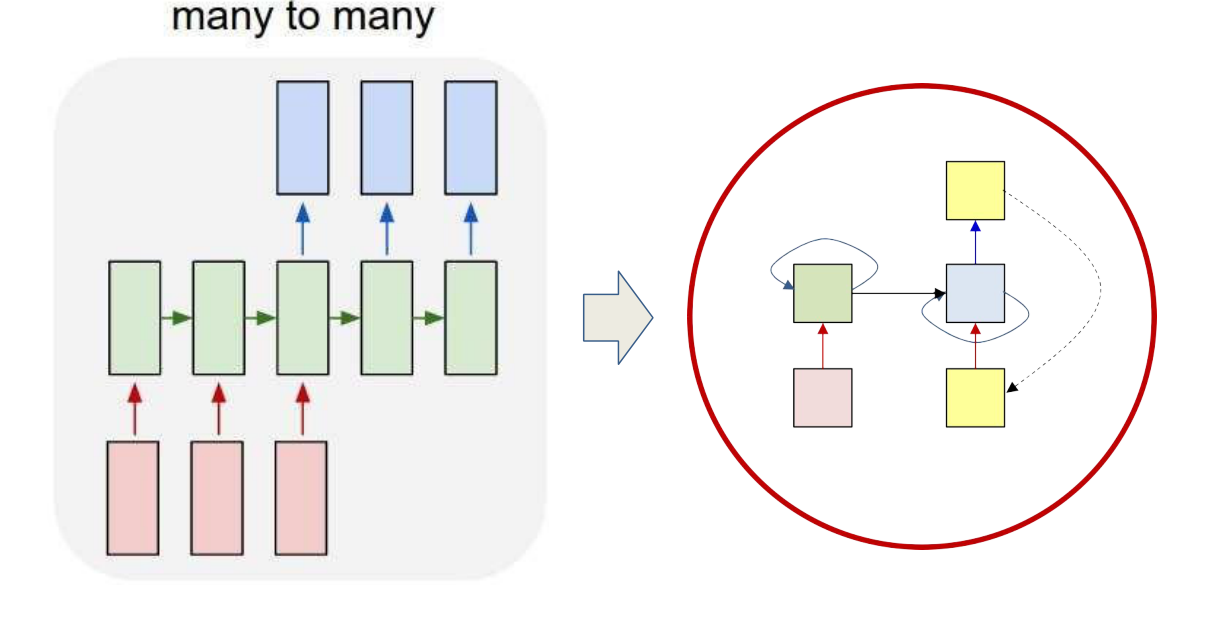
\includegraphics[width=0.35\paperwidth,height=0.35\paperheight,keepaspectratio]{images/seq2seq+attention/seq2seq_rnn_to_recurrent_cell.png}

  {\scriptsize Source: after CMU 11-785 (Spring 2024), Lecture 18: Sequence to Sequence Models \& Attention, slide~7 (RNN-taxonomy panel after A. Karpathy, 2015).}
  \centering
  \begin{itemize}
    \item \textit{Delayed} Sequence to sequence
    \begin{itemize}
    \item Delayed \textit{self-referencing} sequence-to-sequence
    \end{itemize}
  \end{itemize}
\end{frame}

\begin{frame}{The “simple” translation model}
  \centering
  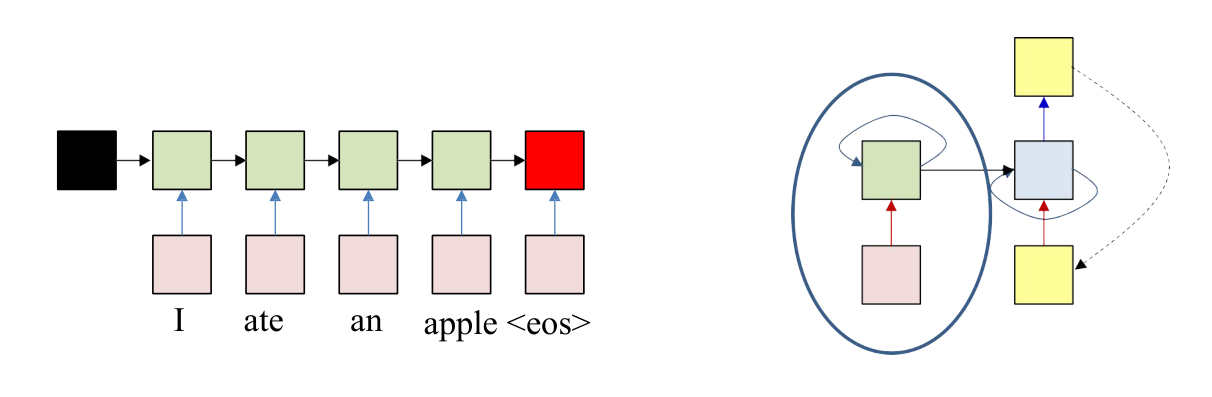
\includegraphics[width=0.35\paperwidth,height=0.35\paperheight,keepaspectratio]{images/seq2seq+attention/seq2seq_encoder_unrolled_with_eos.png}

  {\scriptsize Source: after CMU 11-785 (Spring 2024), Lecture 18: Sequence to Sequence Models \& Attention, slide~8.}
  \begin{itemize}
    \item The input sequence feeds into a recurrent structure 
    \item The input sequence is terminated by an explicit \texttt{<eos>} symbol 
    \begin{itemize}
        \item \textcolor{red}{The hidden activation at the \texttt{<eos>} ``stores'' all information about the sentence} 
    \end{itemize}
\end{itemize}  
\end{frame}

\begin{frame}{The “simple” translation model}
  \centering
  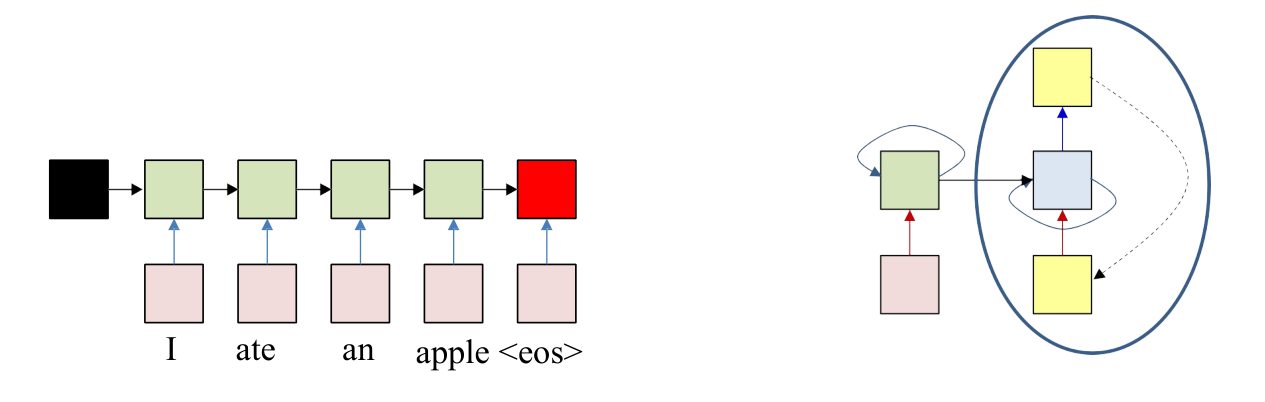
\includegraphics[width=0.35\paperwidth,height=0.35\paperheight,keepaspectratio]{images/seq2seq+attention/seq2seq_encoder_to_recurrent_cell.png}

  {\scriptsize Source: after CMU 11-785 (Spring 2024), Lecture 18: Sequence to Sequence Models \& Attention, slide~9.}
  \begin{itemize}
    \item The input sequence feeds into a recurrent structure 
    \item The input sequence is terminated by an explicit \texttt{<eos>} symbol 
    \begin{itemize}
        \item The hidden activation at the \texttt{<eos>} ``stores'' all information about the sentence 
    \end{itemize}
    \item Subsequently a second RNN uses the hidden activation as initial state, and \texttt{<sos>} as initial symbol, to produce a sequence of outputs
    \begin{itemize}
        \item The output at each time becomes the input at the next time 
        \item Output production continues until an \texttt{<eos>} is produced 
    \end{itemize}
\end{itemize}  
\end{frame}

\begin{frame}{The “simple” translation model}
  \centering
  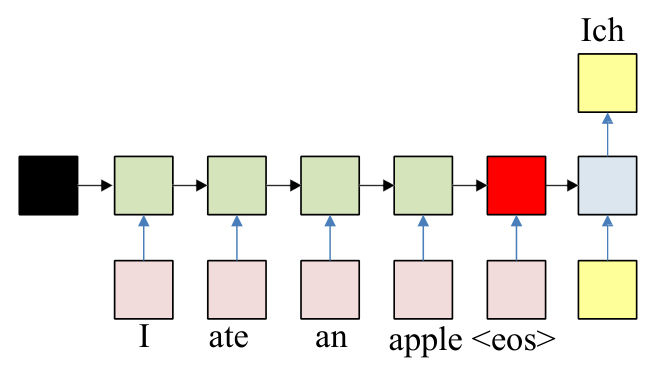
\includegraphics[width=0.35\paperwidth,height=0.29\paperheight,keepaspectratio]{images/seq2seq+attention/seq2seq_decoder_first_word.png}

  {\scriptsize Source: after CMU 11-785 (Spring 2024), Lecture 18: Sequence to Sequence Models \& Attention, slide~10.}
  \begin{itemize}
    \item The input sequence feeds into a recurrent structure
    \item The input sequence is terminated by an explicit \texttt{<eos>} symbol
    \begin{itemize}
        \item The hidden activation at the \texttt{<eos>} ``stores'' all information about the sentence
    \end{itemize}
    \item Subsequently a second RNN uses the hidden activation as initial state to produce a sequence of outputs
    \begin{itemize}
        \item The output at each time becomes the input at the next time
        \item Output production continues until an \texttt{<eos>} is produced
    \end{itemize}
\end{itemize}  
\end{frame}

\begin{frame}{The “simple” translation model}
  \centering
  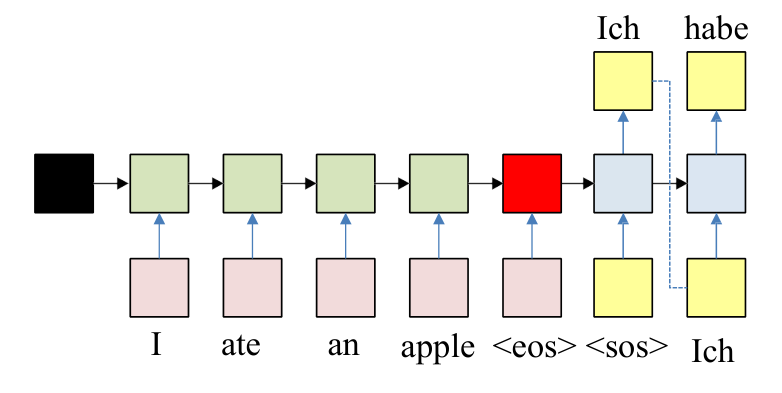
\includegraphics[width=0.35\paperwidth,height=0.29\paperheight,keepaspectratio]{images/seq2seq+attention/seq2seq_decoder_two_words.png}

  {\scriptsize Source: after CMU 11-785 (Spring 2024), Lecture 18: Sequence to Sequence Models \& Attention, slide~11.}
  \begin{itemize}
    \item The input sequence feeds into a recurrent structure
    \item The input sequence is terminated by an explicit \texttt{<eos>} symbol
    \begin{itemize}
        \item The hidden activation at the \texttt{<eos>} ``stores'' all information about the sentence
    \end{itemize}
    \item Subsequently a second RNN uses the hidden activation as initial state to produce a sequence of outputs
    \begin{itemize}
        \item The output at each time becomes the input at the next time
        \item Output production continues until an \texttt{<eos>} is produced
    \end{itemize}
\end{itemize}  
\end{frame}

\begin{frame}{The “simple” translation model}
  \centering
  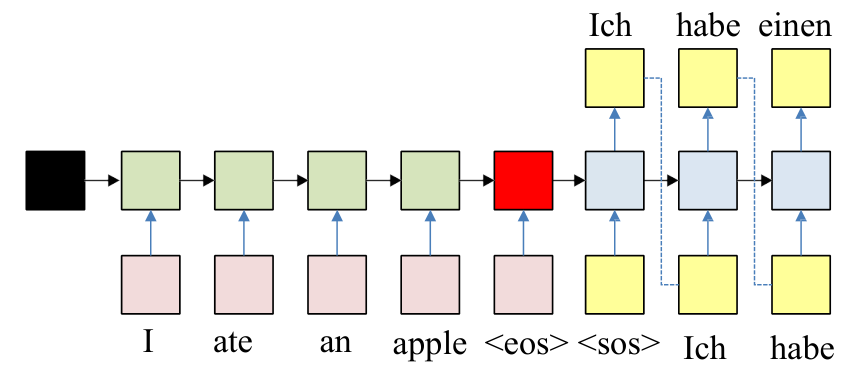
\includegraphics[width=0.35\paperwidth,height=0.29\paperheight,keepaspectratio]{images/seq2seq+attention/seq2seq_decoder_three_words.png}

  {\scriptsize Source: after CMU 11-785 (Spring 2024), Lecture 18: Sequence to Sequence Models \& Attention, slide~12.}
  \begin{itemize}
    \item The input sequence feeds into a recurrent structure 
    \item The input sequence is terminated by an explicit \texttt{<eos>} symbol 
    \begin{itemize}
        \item The hidden activation at the \texttt{<eos>} ``stores'' all information about the sentence 
    \end{itemize}
    \item Subsequently a second RNN uses the hidden activation as initial state to produce a sequence of outputs 
    \begin{itemize}
        \item The output at each time becomes the input at the next time 
        \item Output production continues until an \texttt{<eos>} is produced 
    \end{itemize}
\end{itemize}
\end{frame}

\begin{frame}{The “simple” translation model}
  \centering
  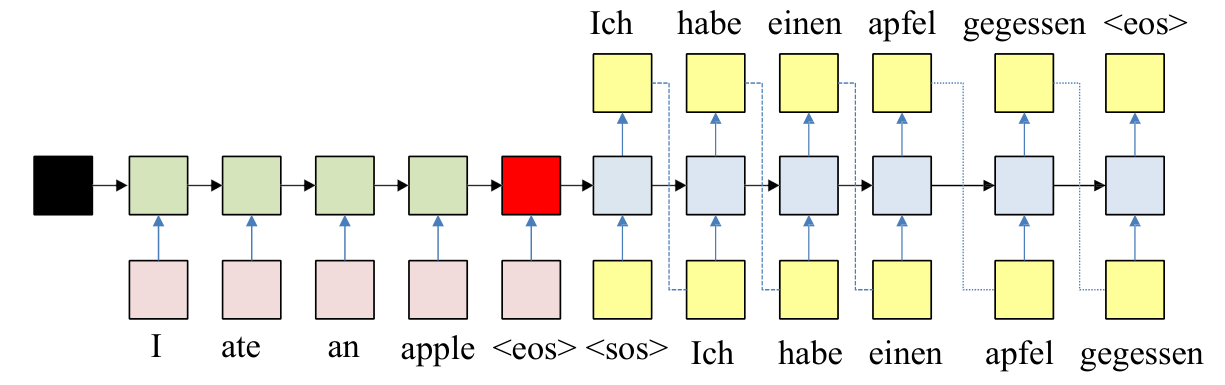
\includegraphics[width=0.35\paperwidth,height=0.29\paperheight,keepaspectratio]{images/seq2seq+attention/seq2seq_decoder_full_output.png}

  {\scriptsize Source: after CMU 11-785 (Spring 2024), Lecture 18: Sequence to Sequence Models \& Attention, slide~13.}
  \begin{itemize}
    \item The input sequence feeds into a recurrent structure 
    \item The input sequence is terminated by an explicit \texttt{<eos>} symbol 
    \begin{itemize}
        \item The hidden activation at the \texttt{<eos>} ``stores'' all information about the sentence 
    \end{itemize}
    \item Subsequently a second RNN uses the hidden activation as initial state to produce a sequence of outputs 
    \begin{itemize}
        \item The output at each time becomes the input at the next time 
        \item Output production continues until an \texttt{<eos>} is produced 
    \end{itemize}
\end{itemize}
\end{frame}

\begin{frame}{The “simple” translation model}
  \centering
  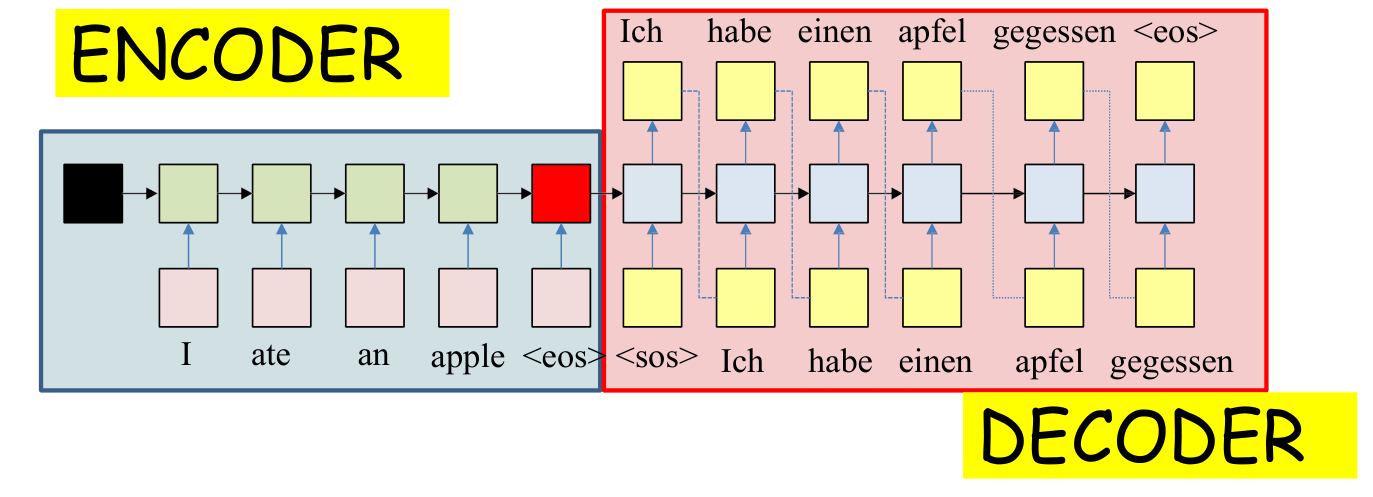
\includegraphics[width=0.35\paperwidth,height=0.35\paperheight,keepaspectratio]{images/seq2seq+attention/seq2seq_encoder_decoder_labeled.png}

  {\scriptsize Source: after CMU 11-785 (Spring 2024), Lecture 18: Sequence to Sequence Models \& Attention, slide~14.}
  \begin{itemize}
    \item The recurrent structure that extracts the hidden representation from the input sequence is the \textbf{encoder} 
    \item The recurrent structure that utilizes this representation to produce the output sequence is the \textbf{decoder}
  \end{itemize}  
\end{frame}